\section{Wzroce projektowe (2) - strukturalne}

\subsection{Adapter (ang. adapter)}

Wzorcem który pozwala na działanie dwóch komponentów o niezgodnych interfejsach nazywany jest adapterem. Jeśli klasa potrzebuje do działania obiektu klasy o określonym interfejsie, natomiast klasa która mogłaby zostać wykorzystana posiada inny, niezgodny interfejs można utworzyć klasę adaptera, która dostosuje interfejsy. Jest on stosowany do zmieniania interfejsu istniejącego kodu.

\begin{figure}[hbt!]
	\centering
	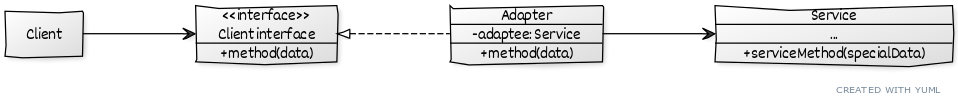
\includegraphics[width=0.9\linewidth]{images/AdapterUml}
	\caption{Diagram UML wzorca Adapter.}
	\label{lab3/fig/AdapterUml}
\end{figure}
%[Client interface]^-.-[Adapter]
%[Adapter]->[Service]
%[Client]->[Client interface]
%
%[Client]
%[<<interface>>Client interface|+method(data)]
%[Adapter|-adaptee: Service|+method(data)]
%[Service|...|+serviceMethod(specialData)]

Wyobraźmy sobie sytuację, w której mamy działający komponent i np. do logowania informacji o swoim działaniu wykorzystuje napisany przez nas zestaw. Klasa logera implementuje określony interfejs i przez ten interfejs klasa kliencka wykorzystuje zestaw do logowania. Jeśli za jakiś czas okażę się konieczne wykorzystanie bardziej rozbudowanego narzędzia np. pakietu NLog, możemy albo zmieniać odwołania w całym kodzie klienckim, albo wykorzystać adapter. W tym przypadku adapterem będzie klasa implementująca interfejs np. \texttt{ILogger} i posiadająca obiekt typu \texttt{NLog.Logger} przekazany np. jako argument konstruktora. Wszystkie metody interfejsu \texttt{ILogger} są przekazywane do odpowiednich metod pakietu \texttt{NLog}. Na napisaniu adaptera wystarczy wstrzyknąć nowo utworzony obiekt do kodu klienckiego bez dodatkowych modyfikacji. Nie będzie również problemem rozszerzyć napisać dodatkowy adapter dla innego pakietu np. Log4N. Ze względu na fakt, że oba adaptery implementują ten sam interfejs można posiadać wiele różne adaptery dla różnych obiektów adaptowanych.

Innym przykładem może być sytuacja w której posiadamy aplikację pobierająca dane z plików tekstowych w formacie \texttt{XML} i dalej je przetwarzającą plus wizualizującą te dane w formie wykresów. W czasem jednak pojawiła się potrzeba, aby dane pobierać z zewnętrznego serwera w formacie \texttt{JSON} korzystając z gotowego zestawu. Jeśli korzystamy z gotowych rozwiązań innych firm nie ma możliwość zmienić interfejsu zestawu pobierającego  dane z serwera. Implementując wykorzystywany wcześniej interfejs możemy przekierowywać żądania od klienta do zewnętrznego zestawu w locie zmieniając format danych z \texttt{XML} na \texttt{JSON}.

Opisana powyżej wersja adaptera jest wersją obiektową tego wzorca. Można się również spotkać z podejście klasowym, wtedy obiekt adaptera zamiast posiadać adaptowany obiekt, może po nim dziedziczyć. Jednak zgodnie z zasadą, aby przekładać kompozycję nad dziedziczenie ten wariant jest rzadziej stosowany. 

% Plusem adaptera klasowego jest możliwość przesłonięcia składowych wirtualnych, abstrakcyjnych. 
% W przypadku C++ stosując adapter klasowy należy publicznie dziedziczyć po klasie Target oraz prywatnie po klasie Adaptee.
% Podejście obiektowe jednak pozwala na działanie jednej kalsy Adapter z wieloma Adaptee



\subsection{Kompozyt (ang. composite)}

Kompozyt łączy obiekty w struktury drzewiaste i pozwala klientom traktować je jak osobne obiekty. Drzewo składa się z dwóch rodzajów elementów liści oraz kontenerów. Kontener może składać się z liści oraz z innych kontenerów. Wzorzec ten powinien być stosowany jeżeli z punktu widzenia klienta nie ma znaczenia czy odwołuje się on do pojedynczego elementu czy drzewiastej struktury. Zazwyczaj klient nie wie z jakiego typu elementu korzysta. Klient będzie ignorował różnice pomiędzy pojedynczymi, a złożonymi obiektami.

Wzorzec Kompozyt wykorzystuje interfejs albo klasę abstrakcyjną do reprezentacji zarówno typów prostych jak i złożonych. Wszystkie one muszą implementować wspólny interfejs albo dziedziczyć po klasie abstrakcyjnej.
 
\begin{figure}[hbt!]
	\centering
	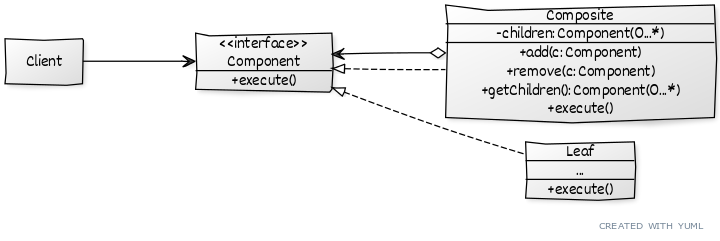
\includegraphics[width=0.8\linewidth]{images/CompositeUml}
	\caption{Diagram UML wzorca kompozyt.}
	\label{lab3/fig/CompositeUml}
\end{figure}
%[Client]->[Component]
%[Component]^-.-[Composite]
%[Composite]<>->[Component]
%[Component]^-.-[Leaf]
%
%[Client]
%[<<interface>>Component|+execute()]
%[Leaf|...|+execute()]
%[Composite|-children: Component(0...*)|+add(c: Component);+remove(c: Component);+getChildren(): Component(0...*);+execute()]

Łatwo można sobie wyobraź drzewo składające się z produktów oraz pudełek (kontenerów) które je przechowują. Zarówno liście jak i kontenery implementują wspólny interfejs. Klient wywołuję metodę np. \texttt{GetPrice()} głównego kontenera (korzenia). Jeśli dzieckiem danego wierzchołka jest liść (produkt ) zwracana jest jego cena, żądanie zostaje obsłużone bezpośrednio. Jeśli natomiast dzieckiem jest inny kontener (obiekt \texttt{Composite}) to przeglądana jest jego zawartość i ponownie w zależności od zawartości podejmowana jest akcja dalszego przeglądania albo zwracania wartości ceny.

Interfejsy graficzne, systemy SCADA zwykle pozwalają na rysowanie złożonych elementów z wielu prostych elementów. Klient zwykle nie chce traktować prostych i złożonych elementów w odmienny sposób. Powoduje do dodatkowe skomplikowanie modułu programu. Klasy \texttt{Line}, \texttt{Rectangle}, \texttt{Text} definiują proste elementy graficzne. Natomiast klasa \texttt{Picture} mogłaby stanowić kontener, w którym były przechowywane proste elementy podrzędne.

Istotne jest to, że istnieje możliwość dodania nowych typów, które mogą być liśćmi drzewa bez zmiany kodu klienta. Jest to właściwość zgodna z zasadą otwarte/zamknięte. Trudne może okazać się znalezienie wspólnego interfejsu dla wszystkim elementów Kompozytu.

Korzystając z wzorca Budowniczy można tworzyć drzewa Kompozytowe.

\subsection{Fasada (ang. facade)}
Jeśli istnieje potrzeba, aby ukryć złożoność biblioteki albo innego zbioru wielu klas można użyć wzorca fasady. Jest to bardzo prosty wzorzec upraszczający sposób w jaki klienci korzystają z współpracujących, zależnych od siebie klas. Udostępnia jednolity interfejs dla zbioru interfejsów z podsystemu. Wykorzystując fasadę klient nie musi tworzyć, ani zarządzać zależnościami pomiędzy obiektami są one przed nim ukryte za interfejsem fasady. Fasada może również służyć za punkt wejścia dla podsystemu w warstwowo podzielonym zestawie.

Fasada pozwala zmniejszyć liczbę obiektów z której korzystają klienci. Dodatkowo wprowadza się luźne powiązanie pomiędzy klientami, a podsystemami. Ułatwione jest wprowadzanie zmian w podsystemach czy zmiana zależności między nimi. 

\begin{figure}[hbt!]
	\centering
	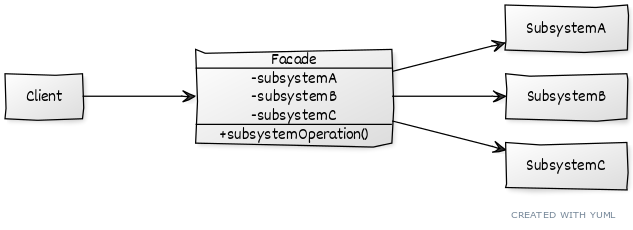
\includegraphics[width=0.8\linewidth]{images/FacadeUml}
	\caption{Diagram UML wzorca Fasada.}
	\label{lab3/fig/FacadeUml}
\end{figure}
%[Client]->[Facade]
%[Facade]->[SubsystemA]
%[Facade]->[SubsystemB]
%[Facade]->[SubsystemC]
%
%[Client]
%[Facade|-subsystemA;-subsystemB;-subsystemC|+subsystemOperation()]
%[SubsystemA]
%[SubsystemB]
%[SubsystemC]

Interfejs udostępniany przez omawiany wzorzec jest zazwyczaj uproszczony, nie posiada wszystkich funkcjonalności, które zapewniają ukrywane przez niego klasy. Dostarczane są jedynie te niezbędne. Jedynie bardziej wymagający klienci będą musieli spojrzeć za fasadę.

Przykładem zastosowania fasady może być proces konwersji materiału wideo. Jest on złożony, wykorzystuje różne klasy do kompresji materiału wideo, miksowania audio, zmiany formatu pliku itp. Klient może potrzebować jedynie uproszczonego interfejsu do konwertowania pliku wideo. Nie muszą go interesować złożone mechanizmy tego procesu. Dlatego zamiast zmuszać klienta do posiadania i zarządzania wieloma klasami, można utworzyć klasę fasady, która te złożoności ukryje. Jeśli w przyszłości część wykorzystywanych klas się zmieni, aktualizacja kodu będzie potrzebna tylko w jednym miejscu, w klasie fasady.

Innym przykładem może być podsystem kompilujący. Klienta nie interesują złożone zależności pomiędzy parserem, preprocesorem, analizatorem semantyki czy optymalizatorem. Autorzy klientów chcą tylko skompilować kod. Jeśli proces kompilacji ukryć w pojedynczej klasie \texttt{Compiler}, bo będzie ona odgrywała rolę fasady. Będzie udostępniać klientom prosty interfejs do kompilacji.
% g++ -Wall -std=c++14 main.cpp -o main.exe //-Wall (all warnings) and -o main.exe instead of a.exe